\chapter{Experimentos, resultados e discussão}
\label{sec::experimentos}

Neste capítulo, mostramos os experimentos e resultados do algoritmo de renderização proposto, bem como as funcionalidades adicionadas ao longo do tempo objetivando a interatividade.

 Na Seção \ref{chap::renderizacao_de_perfis_de_difusao}, apresentamos um ambiente de testes e abordamos a evolução do algoritmo de glifos ODFs feitas nesse trabalho, objetivando a interatividade que culminaram no algoritmo de renderização apresentado no Capítulo \ref{chap::renderizacao_interativa_de_perfis_de_difusao}.
Na Seção \ref{sec::glifos_odf_visualizacao_multimodal}, descrevemos os experimentos e resultados do algoritmo de renderização glifos ODF integrados ao ambiente de visualização multimodal.

%%%%%%%%%%%%%%%%%%%%%%%%%%%%%%%%%%%%%%%%%%%%%%%%%%%%%%%%%%%%%%%%%%%%%%%%%
\section{Ambiente e Dados de Teste}

Todos os experimentos e medições foram feitas em um computador Macbook Pro Retina 13', com processador Intel Core i5 Dual-Core 2.7GHz, processador gráfico integrado Intel Iris Graphics 6100 1536 MB e memória RAM de 8 GB 1867 MHz DDR3.

\todo[inline]{Como são feitas as medidas? Como é estimada a ocupação da memória?}

\textcolor{red}{Foram usados dois conjuntos de dODFs de teste. Um conjunto compreende os dados sintetizados a partir de funções harmônicas esféricas, e outro conjunto são dados obtidos a partir dos exames de ressonância magnética disponíveis no repositório \textit{WU-Minn HCP Retest Data} do \textit{Connectome Project Consortium} \cite{essen2012}. Utilizamos as funções harmônicas esféricas para geração de dados sintéticos, porque os glifos destas funções são conhecidos\footnote{A página https://chem.libretexts.org/@go/page/283935 oferece a visualização das funções harmônicas esféricas em plotagens polares esféricas.}. Isso serviu de suporte para depuração dos códigos.  E usamos os dados reais do \textit{Connectome Project Consortium} por ser o único repositório em que encontramos os volumes de ressonância magnética ponderada em T1 e ponderada em difusão (protocolo HARDI) de um mesmo paciente.}

%Esta classe de funções também é comumente utilizada pela comunidade de pesquisa de métodos de alta ordem em DWI.

\subsection{Dados Sintéticos}

\todo[inline]{Revise o texto.}

 As amostras que geram os glifos são computadas a priori a partir de ODFs computadas a partir de funções harmônicas esféricas, cujo \sout{o} grau das funções varia de zero a três. 

Indexamos as células nas quais os glifos são renderizados como $1$, $2$, ..., $M$, cuja sequência é crescente na ordem esquerda para direita e cima e para baixo, e $M = H^2$. Associamos o conjunto de amostras a serem renderizadas na $j$-ésima $(1 \leq j \leq M)$ célula como $\boldsymbol{R}(j) = [
R(j, \mathbf{n}_1), 
R(j, \mathbf{n}_2), 
R(j, \mathbf{n}_3), ..., 
R(j, \mathbf{n}_N)
]^T$, onde $\mathbf{n}_k$ é o vetor unitário com direção e sentido associado à normal do ponto $P_k$ de uma malha esférica $(\Pi, I)$, onde $\Pi = [P_1, P_2, \dots, P_N]$. $I_{3\tau \times 1}$ é o conjunto de índices que triangulam $\Pi$ afim de gerar a malha esférica, onde $\tau$ é a quantidade de triângulos da malha.%\footnote{Escolhemos esta forma de indexar as variáveis envolvidas para que fique similar à forma utilizada no Capítulo \ref{chap::renderizacao_interativa_de_perfis_de_difusao}.}

Utilizamos dez funções harmônicas esféricas, em que, na Fig. \ref{fig::ambiente_validacao_5}, da esquerda para direita e parte superior para inferior, consistem em: $Re(Y_1^{-1})$,
$Re(Y_1^0)$,
$Im(Y_1^{-1})$,
$Re(Y_2^{-2})$,
$Im(Y_2^{-2})$,
$Re(Y_2^{-1})$,
$Im(Y_2^{-1})$,
$Y_2^0$,
$Y_0^0$ e
$Y_3^0$, onde $Y_l^m$ se refere a harmônica esférica de grau $l$ e ordem $m$. 

As expressões analíticas para as harmônicas esféricas de ordem zero a dois e $Y_3^0$ utilizadas no Capítulo \ref{chap::renderizacao_de_perfis_de_difusao} são:
\begin{equation}
\begin{array}{l}
Y_{0}^{0}(\theta, \varphi)=\frac{1}{2} \sqrt{\frac{1}{\pi}} \\
Y_{1}^{-1}(\theta, \varphi)=\frac{1}{2} \sqrt{\frac{3}{2 \pi}} \sin (\theta) e^{-i \varphi} \\
Y_{1}^{0}(\theta, \varphi)=\frac{1}{2} \sqrt{\frac{3}{\pi}} \cos (\theta) \\
Y_{1}^{1}(\theta, \varphi)=\frac{-1}{2} \sqrt{\frac{3}{2 \pi}} \sin (\theta) e^{i \varphi} \\
Y_{2}^{-2}(\theta, \varphi)=\frac{1}{4} \sqrt{\frac{15}{2 \pi}} \sin ^{2} (\theta) e^{-2 i \varphi} \\
Y_{2}^{-1}(\theta, \varphi)=\frac{1}{2} \sqrt{\frac{15}{2 \pi}} \sin (\theta) \cos (\theta) e^{-i \varphi} \\
Y_{2}^{0}(\theta, \varphi)=\frac{1}{4} \sqrt{\frac{5}{\pi}}\left(3 \cos ^{2} (\theta)-1\right) \\
Y_{2}^{1}(\theta, \varphi)=\frac{-1}{2} \sqrt{\frac{15}{2 \pi}} \sin (\theta) \cos (\theta) e^{i \varphi} \\
Y_{2}^{2}(\theta, \varphi)=\frac{1}{4} \sqrt{\frac{15}{2 \pi}} \sin ^{2} (\theta) e^{2 i \varphi} \\
Y_{3}^{0}(\theta, \varphi)=\frac{1}{4} \sqrt{\frac{7}{\pi}}\left(5 \cos ^{3} (\theta)-3 \cos (\theta)\right)
\end{array}
\end{equation}


\sout{Na Seção \ref{sec::harmonicas_esfericas} do Apêndice, escrevemos a formulação analítica das funções utilizadas.} Fazemos a associação entre cada $\boldsymbol{R}(j)$, a sua respectiva harmônica esférica de acordo com a Tabela \ref{tab::harmonicas_esfericas}, na qual computamos o seu valor absoluto e fazemos a normalização min-max para o intervalo $[0, 1]$ dos valores amostrados\footnote{No caso da harmônica esférica $(Y_0^0)$, que é constante e mapeada em um glifo esférico, normalizamos a função para ser constante igual a um.}, que são pré-computadas na CPU. Fig. \ref{fig::ambiente_validacao} ilustra os glifos no ambiente de teste para diferentes valores de $M$. O cômputo do valor absoluto torna estas funções simétricas em relação ao eixos coordenados, assim como as funções e sinais de difusão.

\begin{table}[ht]
\centering
\begin{tabular}{cc}
$j \mod 10$ & Harmônica Esférica \\ \hline
1 & $Re(Y_1^{-1})$  \\
2 & $Re(Y_1^0)$     \\
3 & $Im(Y_1^{-1})$  \\
4 & $Re(Y_2^{-2})$  \\
5 & $Im(Y_2^{-2})$  \\
6 & $Re(Y_2^{-1})$  \\
7 & $Im(Y_2^{-1})$  \\
8 & $Y_2^0$         \\
9 & $Y_0^0$         \\
0 & $Y_3^0$        
\end{tabular}
\caption{Associação de índice de célula para função harmônica esférica utilizada. Adicionamos o cômputo dos valores absolutos e fizemos a normalização min-max para cômputo de $\boldsymbol{R}(j)$. Os glifos ODF estão ilustrados em Fig. \ref{fig::ambiente_validacao}.}
\label{tab::harmonicas_esfericas}
\end{table}

\label{sec::harmonicas_esfericas}
 A conversão de $\mathbf{\hat{u}} = (u_x, u_y, u_z)$, $|\mathbf{\hat{u}}| = 1$ para o par $(\theta, \varphi)$ é dado por:
 \begin{equation}
     (\theta, \varphi) = (\arccos (u_z), \arctan (\frac{u_y}{u_x}))
 \end{equation}

\subsection{Dados de Ressonância Magnética}

\todo[inline]{Revise o texto.}

\sout{As imagens geradas no experimento foram coletadas}\textcolor{red}{Usamos os dados do repositório} \sout{a partir o} \textit{WU-Minn HCP Retest Data} \textcolor{red}{mantido} pelo \textit{Connectome Project Consortium} \cite{essen2012}.

Os dados de difusão foram adquiridos em um \textit{scanner} Siemens 3T Skyra. A aquisição é \textit{multi-shell} com 90 gradientes de ponderação de difusão para cada \textit{shell} $b = 1000, 2000$ e $3000 s/mm^2$, e estas direções são uniformemente distribuídas nos três \textit{shells}, e adicionalmente foram escaneados 6 aquisições $b0$ para cada \textit{shell}, totalizando 288 volumes. Os dados foram pré-processados com a \textit{pipeline} de pré-processamento para dados de difusão do Human Connectomme Project (HCP) \cite{glasser2013}. A aquisição pré-processada é representada por um volume $145\times 174\times  145$ com espaço entre amostras de $1.25\times 1.25 \times 1.25$mm.

A aquisição anatômica ponderada em T1 foi também pré-processada utilizando a pipeline de pré-processamento do HCP \cite{glasser2013}. Como o seu respectivo DWI, é representada por um volume $145\times 174\times  145$ com espaço entre amostras de $1.25\times 1.25\times 1.25$mm.

As dODFs foram obtidas através do GQI \cite{yeh2010} (Capítulo \ref{chapter::metodos_hardi}) e min-max normalizadas. O fator $\sigma \sqrt{6D}$ que utilizamos é de 0,0239. As amostras foram computadas com base no hemisfério da $8^{a}$ ordem de tesselação do icosaedro e armazenadas na CPU, gerando um total de 321 amostras por \textit{voxel}.

%%%%%%%%%%%%%%%%%%%%%%%%%%%%%%%%%%%%%%%%%%%%%%%%%%%%%%%%%%%%%%%
\section{Experimentos}

Para avaliar o desempenho do algoritmo proposto e sua potencial aplicabilidade em dados reais, dividimos em os experimentos em 3 grupos.

\textcolor{red}{O primeiro grupo de experimentos tem como objetivo validar o impacto das diferentes estratégias adotadas na renderização dos glifos ODFs, quanto à ocupação de memória, ao desempenho temporal e à escalabilidade. Foram usados os dados sintéticos para renderizar os glifos centrados nas $H^2$ células quadradas, em que é particionada} uma janela de dimensões $1200 \times 1200$ \textit{pixels}. \textcolor{red}{Avaliamos comparativamente as 5 diferentes configurações em que diferentes estratégias foram integradas incrementalmente: (1) técnica de indexação e visibilidade; (2) técnica de instanciação; (3) compactação de dados de difusão; (4) coalescência; e (5) multi-resolução.}

\textcolor{red}{O segundo grupo de experimentos procura certificar a interatividade e à escalabilidade do algoritmo de renderização proposto em volumes reais, através da avaliação do tempo de resposta do sistema em relação à variação dos fatores de escala de visualização emulando um ambiente de exploração em que um usuário possa variar a escala do que está investigando sob demanda.}

\textcolor{red}{O terceiro grupo de experimentos tem como objetivo de comparar visualmente os glifos superquádricos e os glifos ODFs apresentados neste trabalho quanto à eficiência na visualização das orientações múltiplas de fibras em amostras obtidas pelo protocolo HARDI de exames de ressonância magnética ponderada em difusão.}

\section{Testes com Dados Sintéticos}
%\section{Funcionalidades adicionadas e ganhos de performance}
\label{chap::renderizacao_de_perfis_de_difusao}

Nesta seção, abordamos \sout{a evolução do }\textcolor{red}{o impacto das diferentes estratégias adotadas no }algoritmo de renderização de glifos ODF \sout{feitas neste mestrado} apresentado no Capítulo \ref{chap::renderizacao_interativa_de_perfis_de_difusao}, objetivando a \sout{interatividade}\textcolor{red}{um melhor desempenho em renderização}.
Nos experimentos variamos a divisão $H$ nos eixos $x$ e $y$ da janela de exibição, de 5 até 100, e a resolução de amostragem, setando a ordem de tesselação do icosaedro entre $2^a$, $4^a$, $8^a$ e $16^a$. Fig. \ref{fig::ambiente_validacao} ilustra a partição da área de janela em 25, 625, 2500 e 10000 células.
 
\begin{figure}[ht]
\centering
\captionsetup[subfloat]{farskip=5pt,nearskip=0pt}
    %!!VER SE ISSO TA CERTO
    \subfloat[H = 5. 25 glifos renderizados] {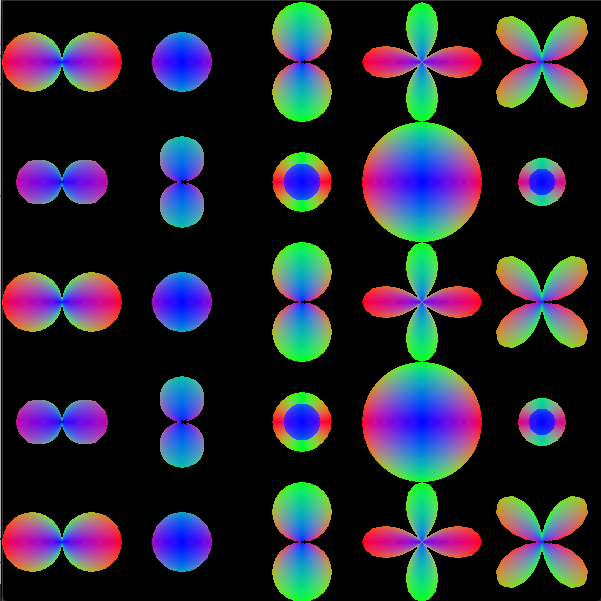
\includegraphics[width=.45\linewidth, angle=0]{figs/Renderizacao_glifos_evolucao/Ilustracao_ambiente/ambiente_5.png}
    \label{fig::ambiente_validacao_5}
    }
    \subfloat[H = 25. 625 glifos renderizados]{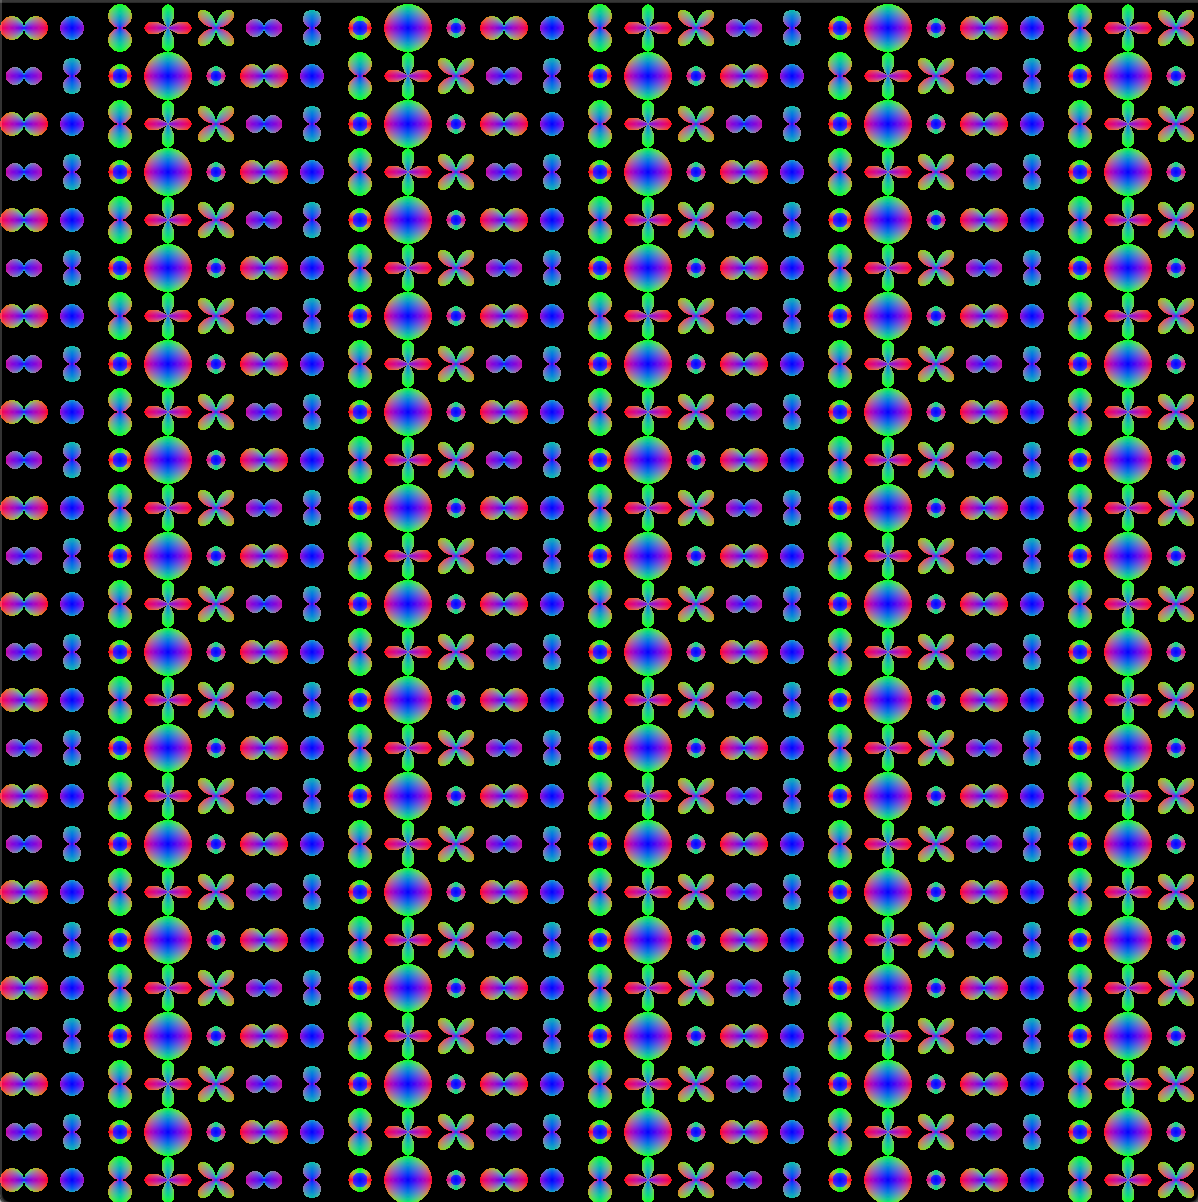
\includegraphics[width=.45\linewidth, angle=0]{figs/Renderizacao_glifos_evolucao/Ilustracao_ambiente/ambiente_25.png}
    \label{fig::ambiente_validacao_25}
    }
    
    \subfloat[H = 50. 2500 glifos renderizados]{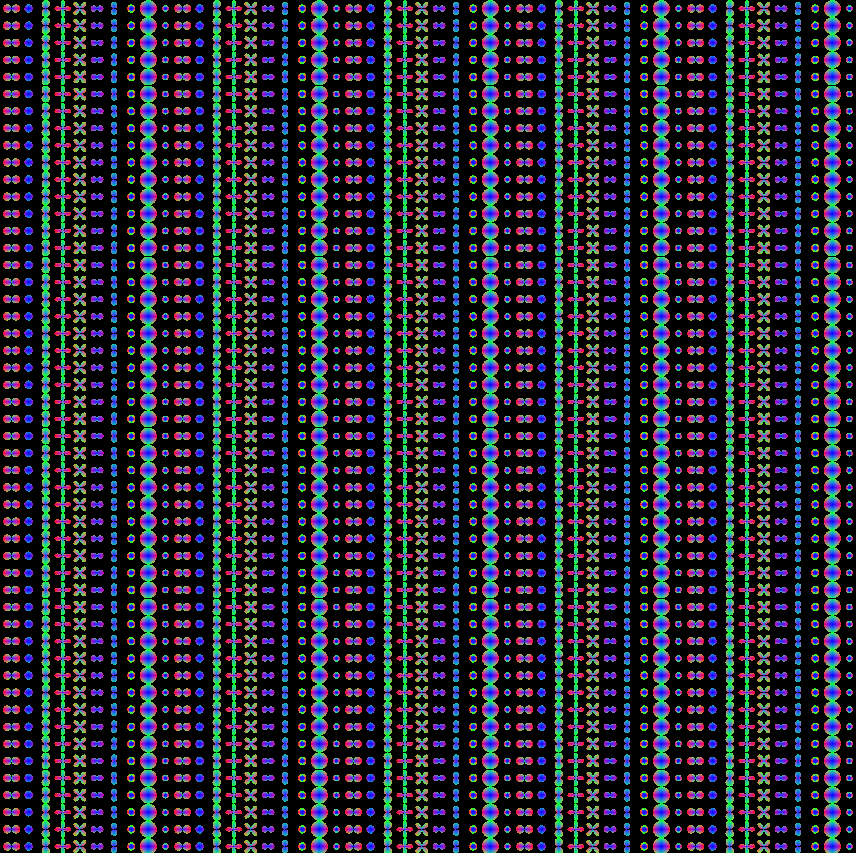
\includegraphics[width=.45\linewidth, angle=0]{figs/Renderizacao_glifos_evolucao/Ilustracao_ambiente/ambiente_50.png}
    \label{fig::ambiente_validacao_50}
    }
    \subfloat[H = 100. 10000 glifos renderizados]{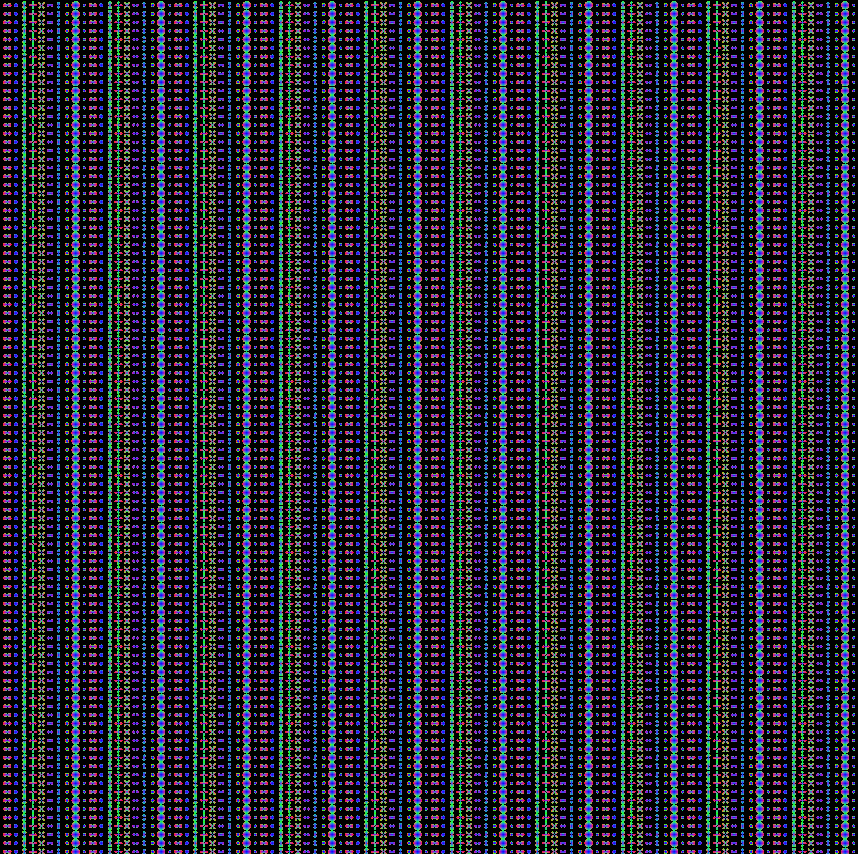
\includegraphics[width=.45\linewidth, angle=0]{figs/Renderizacao_glifos_evolucao/Ilustracao_ambiente/ambiente_100.png}
    \label{fig::ambiente_validacao_100}
    }
     \caption{Ambiente de avaliação do algoritmo de renderização para ODFs. As cores dos glifos referenciam a direção dos eixos de acordo com a Eq. \ref{eq::cor_glifo}.}
    %\hfill
    \label{fig::ambiente_validacao}
\end{figure}


%Na Seção \ref{sec::ambiente_teste}, descrevemos o ambiente de teste que implementamos para fazer a validação  de todas as funcionalidades adicionadas no algoritmo de renderização.

%Na Seção \ref{sec::primeiro_prototipo}, descrevemos o primeiro protótipo do algoritmo, onde o utilizamos na infraestrutura do ambiente de visualização multimodal para renderização dos glifos. Inicialmente, o protótipo consistiu em uma ferramenta visual para visualização de dados de ODFs em seus respectivos \textit{voxels}.

\subsection{Descrição}

\textcolor{red}{Para realizar este grupo de experimentos, desativamos as funções de instanciação, compactação de dados de difusão, coalescência e multi-resolução, e coletamos o tempo médio que se levou para renderizar . Depois fomos reativando essas funções incrementalmente, na sequência de instanciação, compactação, coalescência e multi-resolução, para coletar o mesmo conjunto de dados para análises comparativas.} 

\textcolor{red}{Na primeira série deste experimento são enviados integralmente, em cada interação, não só os $N$ valores correspondentes às probabilidades de difusão em $N$ direções de cada um dos $M$ \textit{vóxeis} visíveis, como também as $N$ direções ($N \times 3$ valores escalares) dos $M$ vóxeis visíveis e $M$ vetores de deslocamento ($M \times 3$ valores escalares). Nesta série armazenamos cada probabilidade de difusão no componente R de um \textit{texel} da textura. Portanto, a quantidade efetiva do espaço de memória alocada para cada probabilidade de difusão são 4 componentes RGBA que correspondem a 4 valores escalares. Substituindo $N$ pela Eq. \ref{eq::icosphere_vertices}, podemos exprimir a quantidade de valores escalares envolvidos na representação dos dados dos $M$ glifos de nível de amostragem de ordem $t$ pela expressão}
\begin{equation}
\label{eq::mem_odfs_1}
    \mathscr{N} =  M \times 3 + M \times (N \times 7) = M \times (3+((10 \times t^2) \times 7)).
\end{equation}
\textcolor{red}{Se cada valor escalar ocupar 4 \textit{bytes}, o volume de dados envolvidos em cada interação é $(M times (3+((10 \times t^2) \times 4)) \times 4)$.}

\textcolor{red}{Aplicando a instanciação na segunda série deste experimento, só é necessário enviar uma vez os vértices/vetores normais da malha esférica ($N \times 3$ valores escalares) e $M$ instâncias de vetores de deslocamento (3 valores escalares) e $N$ probabilidades de difusão (1 valor escalar). Isso reduz o volume de dados para}
\begin{equation}
\label{eq::mem_odfs_2}
    \mathscr{N} =  (N \times 3) + M \times 3 + M \times N \times 4 =  ((10 \times t^2) \times 3) + M \times (3+(10 \times t^2)) \times 4.
\end{equation}

\textcolor{red}{Na terceira série do experimento, ao explorarmos a propriedade de simetria das funções de densidade de orientações e a característica do algoritmo de tesselação que usamos, podemos reduzir para metade a quantidade de probabilidades de difusão associadas às $N$ direções, ficando o volume total de dados em}
\begin{equation}
\label{eq::mem_odfs_3}
    \mathscr{N} =  (N \times 3) + M \times 3 + M \times \frac{N}{2} \times 4 =  ((10 \times t^2) \times 3) + M \times (3+(5 \times t^2)) \times 4.
\end{equation}

\textcolor{red}{Na quarta série do experimento, procuramos otimizar o uso da memória de textura compactando 4 valores de probabilidades de difusão num \textit{texel}, propiciando acessos coalescentes. Com isso, o volume da dados envolvidos na representação dos glifos visíveis fica em}
\begin{equation}
\label{eq::mem_odfs_4}
    \mathscr{N} =  (N \times 3) + M \times 3 + M \times \lceil \frac{N}{2*4} \rceil \times 4 =  ((10 \times t^2) \times 3) + M \times \lceil \frac{(3+(5 \times t^2))}{4} \rceil \times 4.
\end{equation}

\textcolor{red}{Finalmente, na quinta série do experimento ativamos o chaveamento automático da ordem $t$ de tesselação do icosaedro em função do valor $max_p$ (Seção \ref{malha_esferica}, de forma que o volume de dados $\mathscr{N}$ passa a variar com $t$ conforme a Eq. \ref{eq::mem_odfs_4}.}

Para evitar o desperdício de memória e mal uso do cache da GPU, enviamos $\boldsymbol{\mathscr{R}}$ como uma textura de formato RGBA, de tamanho $\lceil \frac{N/2}{4}\rceil \times M$ em que agrupamos os valores escalares da $j$-ésima coluna em sequência de quatro em quatro. Se $N/2$ não é divisível por quatro, é necessária a inserção de linhas com valores \textit{dummy} em $\boldsymbol{\mathscr{R}}$ afim de completar a divisibilidade por quatro, para que cada coluna da matriz possa ser acessada via índice de instância.

Assim, em cada \textit{texel} há quatro amostras de ODF que escalonam 8 pontos da malha esférica. No Capítulo \ref{chap::renderizacao_interativa_de_perfis_de_difusao}, a Fig. \ref{fig::texelfetch} ilustra a forma que o \textit{lookup} é feito, onde neste contexto $j = d_j$. O argumento da função \textit{texelFetch} para a $j$-ésima instância se torna as coordenadas não-normalizadas $(j, \lfloor \frac{Vertex\_ID}{8} \rfloor)$ e o acesso do ponto processado ao seu respectivo valor de ODF min-max normalizado, considerando que as componentes R, G, B e A são mapeados nos índices 0, 1, 2 e 3 nos \textit{texels} é mapeado por $\lfloor Vertex\_ID \mod{8}/2 \rfloor$.
 
\subsection{Resultados}

\todo[inline]{Revise o texto e, principalmente, as legendas para que fiquem coerentes com o restante do texto. Diminua um pouco os gráficos ... ou a legenda ...  Pode ser que caibam 2 figuras por página.}

As medidas de tempo, em fps, em função da quantidade de glifos estão sintetizados no gráfico da Fig. \ref{fig::FPS_prototipo_1}. A configuração de renderização é a mais próxima da abordagem \citeonline{shattuck2008}. A similaridade reside em que os vértices dos glifos são computados na CPU, mas, enquanto na nossa abordagem, as amostras já são pré-computadas, \citeonline{shattuck2008} as computa na CPU em tempo de execução a partir de funções base.

\begin{figure}[H]
    \centering
    %\rule{6cm}{3cm}
    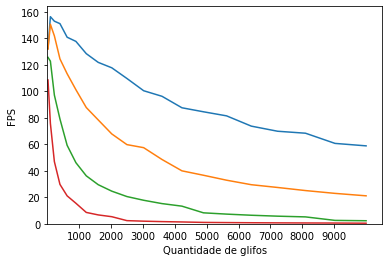
\includegraphics[width=.65\linewidth, angle=0]{figs/Renderizacao_glifos_evolucao/FPS_prototipo1_Geral.png}
    \caption{FPS $\times$ quantidade de glifos renderizada do primeiro protótipo. As cores azul, laranja, verde e vermelha correspondem a geometria base gerada pela $2^{a}$ $4^{a}$, $8^{a}$ e $16^{a}$ ordem de tesselação do icosaedro, respectivamente. Suas quantidades de vértices e triângulo são computadas nas Eq. \ref{eq::icosphere_vertices} e \ref{eq::icosphere_triangulos}, respectivamente.}
    \label{fig::FPS_prototipo_1}
\end{figure}

Fig. \ref{fig::FPS_prototipo_2} mostra de forma comparativa as medidas de tempo, em fps, da configuração de rendering da segunda série de experimentoe em relação à primeira série (Fig. \ref{fig::FPS_prototipo_1}).

\begin{figure}[H]
\centering
\captionsetup[subfloat]{farskip=5pt , nearskip=0pt}
    %!!VER SE ISSO TA CERTO
    \subfloat[Tesselação de $2^a$ ordem] {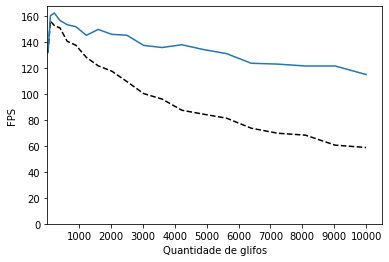
\includegraphics[width=.45\linewidth, angle=0] {figs/Renderizacao_glifos_evolucao/Prototipo2/prototipo_2_42.png}
    \label{fig::FPS_prototipo_2_42}
    }
    \subfloat[Tesselação de $4^a$ ordem] {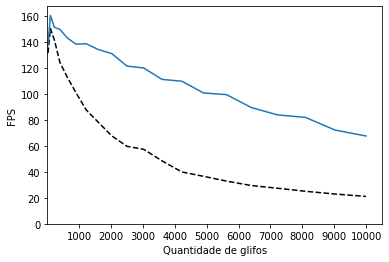
\includegraphics[width=.45\linewidth, angle=0]{figs/Renderizacao_glifos_evolucao/Prototipo2/prototipo_2_162.png}
    \label{fig::FPS_prototipo_2_162}
    }
    
    \subfloat[Tesselação de $8^a$ ordem] {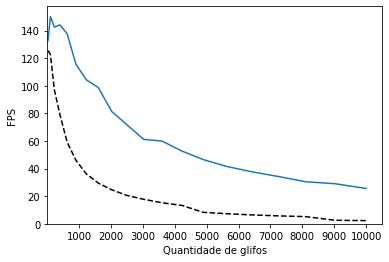
\includegraphics[width=.45\linewidth, angle=0]{figs/Renderizacao_glifos_evolucao/Prototipo2/prototipo_2_642.png}
    \label{fig::FPS_prototipo_2_642}
    }
    \subfloat[Tesselação de $16^a$ ordem] {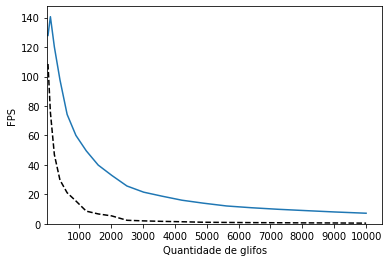
\includegraphics[width=.45\linewidth, angle=0]{figs/Renderizacao_glifos_evolucao/Prototipo2/prototipo_2_2562.png}
    \label{fig::FPS_prototipo_2_2562}
    }
     \caption{FPS $\times$ Quantidade de glifos para diferentes tesselações do icosaedro. A linha preta ilustra o FPS do primeiro protótipo, enquanto a linha azul mostra o FPS da utilização da instanciação da GPU.}
    %\hfill
    \label{fig::FPS_prototipo_2}
\end{figure}

Fig. \ref{fig::FPS_prototipo_3} traz de forma comparativa o gráfico de desempenho do algoritmo de renderização configurada para a terceira série de experimentos em relação ao gráfico apresentado na Fig. \ref{fig::FPS_prototipo_2}.

\begin{figure}[H]
\centering
\captionsetup[subfloat]{farskip=5pt,nearskip=0pt}
    %!!VER SE ISSO TA CERTO
    \subfloat[Tesselação de $2^a$ ordem] {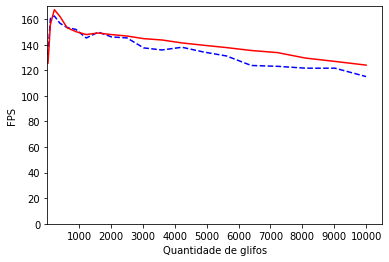
\includegraphics[width=.45\linewidth, angle=0]{figs/Renderizacao_glifos_evolucao/Prototipo3/prototipo_3_42.png}
    \label{fig::FPS_prototipo_3_42}
    }
    \subfloat[Tesselação de $4^a$ ordem] {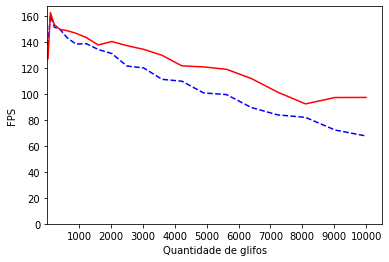
\includegraphics[width=.45\linewidth, angle=0]{figs/Renderizacao_glifos_evolucao/Prototipo3/prototipo_3_162.png}
    \label{fig::FPS_prototipo_3_162}
    }
    
    \subfloat[Tesselação de $8^a$ ordem] {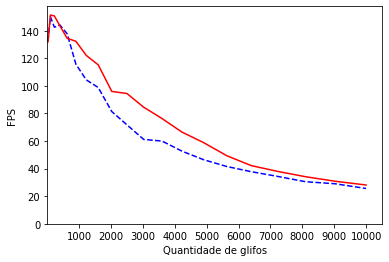
\includegraphics[width=.45\linewidth, angle=0]{figs/Renderizacao_glifos_evolucao/Prototipo3/prototipo_3_642.png}
    \label{fig::FPS_prototipo_3_642}
    }
    \subfloat[Tesselação de $16^a$ ordem] {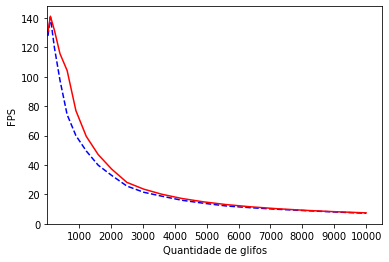
\includegraphics[width=.45\linewidth, angle=0]{figs/Renderizacao_glifos_evolucao/Prototipo3/prototipo_3_2562.png}
    \label{fig::FPS_prototipo_3_2562}
    }
     \caption{FPS $\times$ Quantidade de glifos para diferentes tesselações do icosaedro. A linha pontilhada azul ilustra o FPS do segundo protótipo, enquanto a linha vermelha mostra o FPS quando tomamos vantagem da simetria das ODF.}
    %\hfill
    \label{fig::FPS_prototipo_3}
\end{figure}

Fig. \ref{fig::FPS_prototipo_4} traz de forma comparativa o FPS gerado pela renderização configurada para a quarta série dos experimentos, que apresenta uma nova organização de $\boldsymbol{\mathscr{R}}$, com os gráficos da Fig. \ref{fig::FPS_prototipo_3}.

\begin{figure}[H]
\centering
\captionsetup[subfloat]{farskip=5pt,nearskip=0pt}
    %!!VER SE ISSO TA CERTO
    \subfloat[Tesselação de $2^a$ ordem] {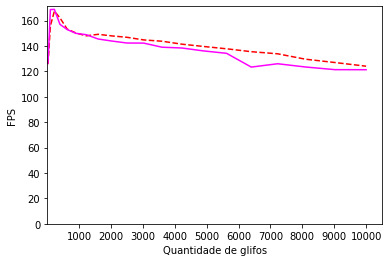
\includegraphics[width=.45\linewidth, angle=0]{figs/Renderizacao_glifos_evolucao/Prototipo4/prototipo_4_42.png}
    \label{fig::FPS_prototipo_4_42}
    }
    \subfloat[Tesselação de $4^a$ ordem] {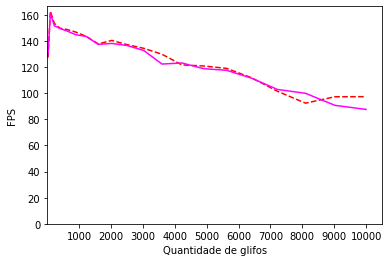
\includegraphics[width=.45\linewidth, angle=0]{figs/Renderizacao_glifos_evolucao/Prototipo4/prototipo_4_162.png}
    \label{fig::FPS_prototipo_4_162}
    }
    
    \subfloat[Tesselação de $8^a$ ordem] {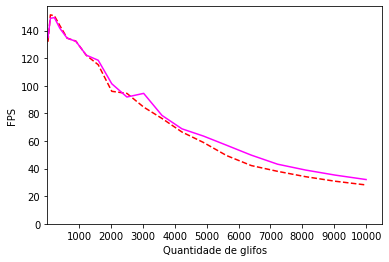
\includegraphics[width=.45\linewidth, angle=0]{figs/Renderizacao_glifos_evolucao/Prototipo4/prototipo_4_642.png}
    \label{fig::FPS_prototipo_4_642}
    }
    \subfloat[Tesselação de $16^a$ ordem] {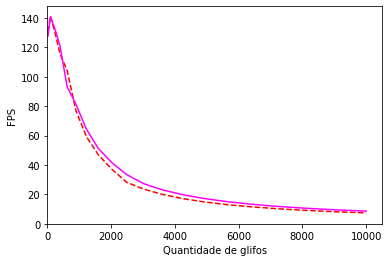
\includegraphics[width=.45\linewidth, angle=0]{figs/Renderizacao_glifos_evolucao/Prototipo4/prototipo_4_2562.png}
    \label{fig::FPS_prototipo_4_2562}
    }
     \caption{FPS $\times$ Quantidade de glifos para diferentes tesselações do icosaedro. A linha pontilhada vermelha ilustra o FPS do terceiro protótipo, enquanto a linha magenta mostra o FPS do uso das componentes RGBA dos \textit{texels} da memória de textura.}
    %\hfill
    \label{fig::FPS_prototipo_4}
\end{figure}

\subsection{Discussões}

\todo[inline]{Revise e adicione comentários sobre escalabilidade para que faça sentido as medidas de tantos números de glifos.}

Na Seção \ref{sec::adaptatividade_de_resolucao}, introduzimos a adaptabilidade na resolução como uma função da máxima quantidade de \textit{pixels} contidos em um único \textit{voxel}, o que é algo intrínseco à métricas do ambiente de visualização multimodal. A validação da inserção deste tópico está nos resultados mostrados na Tabela \ref{tab::glyph_info_experiment}, no qual comparamos com o algoritmo de renderização de glifos ODF integrado ao ambiente de visualização multimodal onde a resolução dos glifos é fixa e derivada da $8^a$ ordem de tesselação do icosaedro, que está anotada na Tabela \ref{tab::glyph_info_experiment_fixed}.

%As medições foram feitas em um computador Macbook Pro Retina 13', com processador Intel Core i5 Dual-Core 2.7GHz, processador gráfico integrado Intel Iris Graphics 6100 1536 MB e memória RAM de 8 GB 1867 MHz DDR3. 
\textcolor{red}{A configuração de renderização na primeira série dos experimentos} gera um tráfego de dados excessivo entre CPU-GPU. Observe que a quantidade de dados por glifo consiste em: $N$ vértices de glifos, $3\tau$ conjunto de índices e $N$ coordenadas de translação. Codificando os vértices e coordenadas de translação em \textit{floats} e o conjunto de índices como inteiro sem sinal, onde cada um destes tipos possui quatro bytes, temos um tráfego CPU-GPU de \todo{Veja se está consistente com o que foi derivado antes.}\textcolor{magenta}{$24N + 12\tau$} bytes por glifo. Adicionalmente, há uma redundância excessiva na quantidade de dados referentes a translação, e as operações de geração de glifos através do escalonamento dos pontos da esfera podem ser paralelizados, o que torna o uso da GPU para seu cômputo uma potencial vantagem. 
Observe \textcolor{red}{Fig. \ref{fig::FPS_prototipo_1}} que mesmo com o tráfego de dados excessivo, foi possível obter uma taxa de quadros razoável com as subdivisões de $2^a$ e $4^a$ ordem.

Note \textcolor{red}{na Fig. \ref{fig::FPS_prototipo_2}} que o tráfego de dados CPU-GPU cai drasticamente \textcolor{red}{para a configuração da segunda série de experimentos}. Para cada glifo, $N$ valores escalares de ODF são enviados a GPU, adicionalmente, conseguimos sintetizar as coordenadas de translação em um atributo único por glifo, e o conjunto de índices é apenas enviado uma vez, o que elimina o tráfego de dados relacionado a esta variável. Assim, o tráfego de dados por glifo cai para $N + 3$ \textit{floats}, totalizando $4N + 12$ \textit{bytes}. Adicionalmente, a malha esférica base é escalonada para gerar o glifo de forma paralela na GPU.

Note também que, para $8^a$ e $16^a$ ordem de tesselação, o FPS mais que dobra para milhares de glifos renderizados. Observe também que neste ambiente, conseguimos renderizar mais de 3000 glifos em taxas interativas \cite{nielsen1994} a partir da malha suave gerada pela $16^a$ ordem de tesselação do icosaedro. O uso de renderização por instâncias e a diminuição do tráfego de dados de amostras de ODF para apenas amostras escalares enviadas como textura foi o ponto mais crucial neste trabalho rumo a interatividade.

\textcolor{red}{Para a configuração da terceira série de experimentos o volume de dados referente aos dados de difusão é reduzido para metada na representação. }
Observe que esta otimização faz o tráfego de dados CPU-GPU ser reduzido de $N + 3$ para $N/2 + 3$ \textit{floats}, totalizando $2N + 12$ bytes. Em termos de performance, observe em Fig. \ref{fig::FPS_prototipo_3_642} e \ref{fig::FPS_prototipo_3_2562} que aproximadamente 4900 e 1225 glifos puderam ser renderizados a 60 FPS para $8^a$ e $16^a$ ordem de tesselação, enquanto na abordagem em que não tomamos vantagem da simetria, 3600 e 900 puderam ser gerados.
Por outro lado, observe que os maiores ganhos de performance ocorrem na faixa que compreendem 600 a 1600 glifos para $16^a$ ordem de tesselação e 2400 até 5000 glifos para para $8^a$ ordem, no qual, nesta região, há um ganho em FPS acima de 20\%.

Note que as componentes B, G e A do \textit{texel} são alocadas, setadas para valores padrão e não são utilizadas\footnote{Informações sobre a alocação de memória em uma textura de formato RED e RGBA podem ser encontradas em https://www.khronos.org/registry/OpenGL-Refpages/gl4/html/glTexImage2D.xhtml}. Adicionalmente, as componentes R, G, B e A na memória de textura em cada \textit{texel} estão em sequência na GPU e nesta abordagem, as amostras que sintetizam o glifo estão espaçadas em 3 \textit{floats}. Neste leiaute de memória, no qual os coeficientes de ODF não estão em sequência, alocamos memória em excesso da GPU para valores não utilizados (componentes B, G e A de cada \textit{texel}) e não utilizamos o cache da GPU de forma ótima.

Observe que \sout{este}\textcolor{red}{o} procedimento \textcolor{red}{da quarta série de experimentos} faz o tráfego de dados CPU-GPU ser sutilmente aumentado para $N/2 + 3 + (4 -N/2 \mod{4})$ \textit{floats} por glifo, mas a quantidade de memória alocada para $\boldsymbol{\mathscr{R}}$ na GPU cai para aproximadamente um quarto em comparação à abordagem anterior.

Observa-se que há um aumento em FPS quando milhares de glifos são renderizados a partir das malhas da $8^a$ e $16^a$ ordem de subdivisão. Na subdivisão de ordem 8, o ganho em FPS é acima de 10\% para mais de 5600 glifos.% Na subdivisão de ordem 16, o ganho de FPS é cerca de 10\% para 1600 glifos renderizados e se estabiliza na faixa de 15\% para mais de 5600 glifos renderizados.
Por outro lado, a diferença é desprezível quando a quantidade de glifos renderizados é menor que 1000 para estas malhas e totalmente desprezível quando utilizamos as tesselações de ordem dois e quatro.

\section{Testes com Dados Reais}
\label{sec::testes_dados_reais}

\textcolor{red}{Neste grupo de experimentos avaliamos o potencial do algoritmo de renderização proposto na implementação de um ambiente de exploração, sob diferentes fatores de escala de visualização, das amostras de difusão dos exames imagiológicos. Elaboramos um experimento em que coletamos os tempos médios de renderização de uma mesma cena variando apenas os fatores de escala de visualização para analisarmos a capacidade adaptativa do algoritmo a diferentes fatores de escala e o seu efeito tanto em tempos de resposta quanto na qualidade dos glifos visualizados.}

\todo[inline]{Revise o texto. Para este experimento, proponho analisar a relação fator de escala (número de glifos) $\times$ tempo.}

Com o objetivo de evidenciar a diferença na resolução e quantidade de triângulos nas transições das malhas esféricas base, fizemos um experimento em que \sout{interagimos com o ambiente de visualização multimodal em que modificamos} ajustamos o fator de escala na visualização tal que o $max_p$ mensurado esteja no limite da troca da malha esférica utilizada no glifo. Fig.  \ref{fig::multimodal_teste_zoom} ilustra experimento.

\subsection{Descrição}

\todo[inline]{Revise o texto: Como você gerou dODFs a partir de DWIs? Quais volumes que você selecionou do repositório do consórcio? Como você planejou o experimento para analisar o desempenho em tempo e a qualidade dos glifos em mostrar as múltiplas configurações de fibras em voxels.}

As dODFs foram obtidas através do GQI \cite{yeh2010} (Capítulo \ref{chapter::metodos_hardi}) e min-max normalizadas. O fator $\sigma \sqrt{6D}$ que utilizamos é de 0,0239. As amostras foram computadas com base no hemisfério da $8^{a}$ ordem de tesselação do icosaedro e armazenadas na CPU, gerando um total de 321 amostras por \textit{voxel}.

\todo[inline]{Qual ângulo de visão do volume foi selecionado para testes?}
Mensuramos o tempo de performance da renderização multimodal de glifos para ODF. O número de glifos é modificado pela mudança do fator de \textit{zoom}. Evidentemente que, maior o fator de \textit{zoom}, menor a quantidade de glifos, maior é a ocupância dos \textit{voxels} na tela, o que aumenta a resolução do glifos. A resolução da janela de saída é de $850\times 850$ e o número de glifos visíveis varia de 12 e 13205. 

\textcolor{red}{Para avaliar a eficácia dos glifos no discernimento das configurações de múltiplas direções de fibras dentro de um voxel, procuramos visualizar as funções dODFs em algumas das regiões destacadas por \citeonline{descoteaux2015} com uso dos glifos propostos. Mais especificamente, as regiões selecionadas são as destacadas na Fig. ...: ....}

\subsection{Resultados}
\label{ssec::reais_resultados}

\todo[inline]{Revise o texto. Eu tentaria uniformizar o contexto das imagens para que se possa desenvolver uma linha de raciocínio em cima de mesmos objetos.}

\textcolor{red}{Variando os fatores de escala de 1.51 a 92,27 geramos uma série de imagens. \todo{Eu mostraria o conteúdo da janela e geraria images de mesmo tamanho.}Na Fig. \ref{fig::multimodal} são ilustradas duas delas.}

\begin{figure}[H]
\centering
\captionsetup[subfloat]{farskip=0pt,nearskip=0pt}
    \subfloat[Fatia coronal de um MRI T1 co-registrado com DWI. A malha esférica base corresponde a $2^a$ ordem de tesselação do icosaedro.]{\makebox[1.2\width]{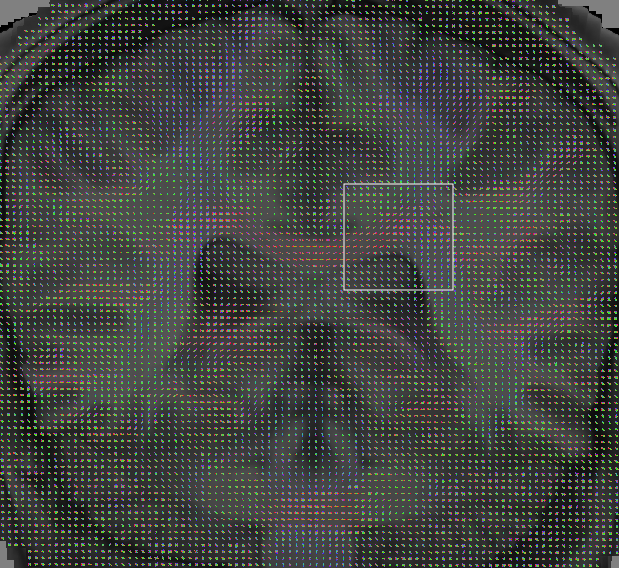
\includegraphics[width=.60\linewidth, angle=0]{figs/Esquema_Glifo/LowResImgHighlighted.png}}
    \label{fig::multimodal_lowres}
    }
    \hspace{1pt}
    
    \subfloat[Cruzamento entre fibras de corpo caloso (esquerda-direita), \textit{corona radiata} (descendente-ascendente) e fascículo longitudinal superior (anteroposterior - normal ao plano da página). A malha esférica base é a $8^a$ ordem de tesselação do icosaedro.] {\makebox[2.0\width]{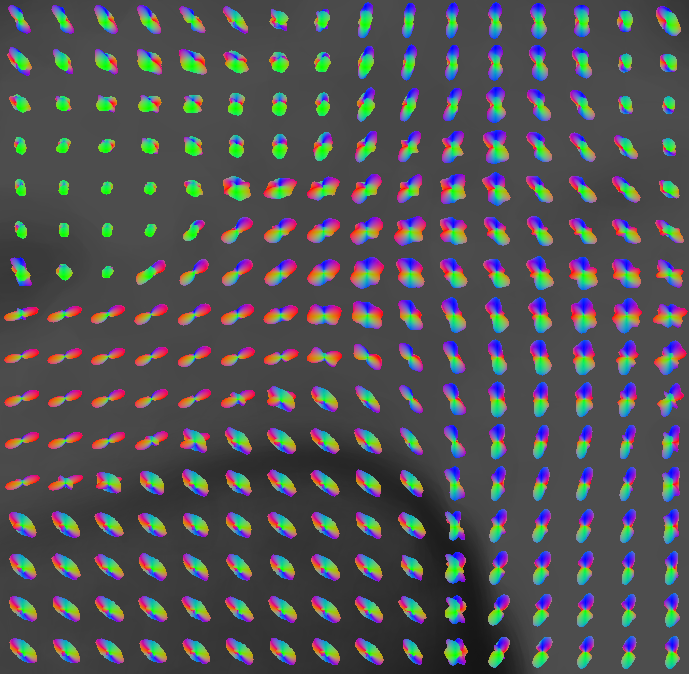
\includegraphics[width=.45\linewidth, angle=0]{figs/Esquema_Glifo/HighResImg.png}
    \label{fig::multimodal_highres}}
    }
    \caption{Glifos ODF integrados ao ambiente de visualização multimodal para MRI. A imagem se refere a um MRI T1 cor-registrado a o seu respectivo DWI. \ref{fig::multimodal_highres} corresponde a região dentro do contorno de cor branca em \ref{fig::multimodal_lowres}.}
    \label{fig::multimodal}
\end{figure}

\textcolor{red}{Certificamos ainda que para fatores de escala baixos são imperceptíveis visualmente as diferenças entre os glifos gerados a partir de icosaedros de distintas ordens de tesselação, como ilustram as Figs. \ref{fig::qualidade_visual_longe_lowres} e \ref{fig::qualidade_visual_longe_highres}. Na Fig. \ref{fig::qualidade_visual_longe_lowres} são renderizados os glifos obtidos a partir de icosaedros de $2^a$ ordem (??? direções) e na Fig. \ref{fig::qualidade_visual_longe_highres}, os da $8^a$ ordem de tesselação (??? direções). }

 \begin{figure}[H]
 %\subfigcapskip = -5pt
     \centering
     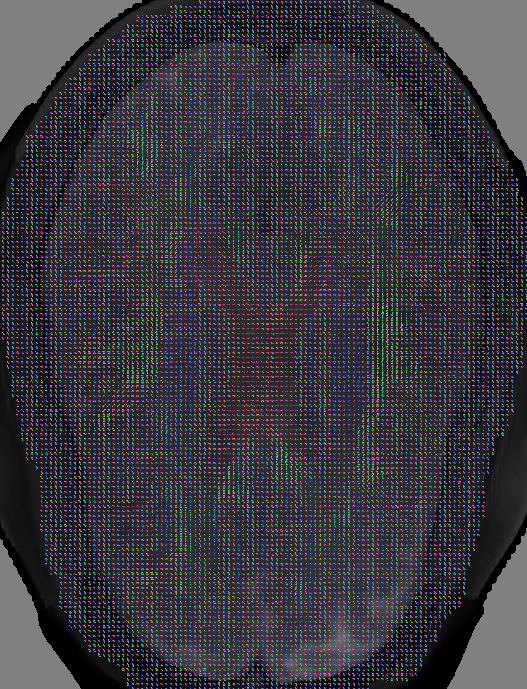
\includegraphics[width=1.0\linewidth, angle=0]{figs/Renderizacao_glifos_evolucao/Adaptividade-multimodal/Fatia_42.png}
      \caption{13205 glifos renderizados sobre um volume \textit{ray-casted}. O glifo é sintetizado a partir da malha esférica obtida pela tesselação de $2^a$ ordem do icosaedro.}
       \label{fig::qualidade_visual_longe_lowres}
  %   \hspace{1pt}
 \end{figure}
 
  \begin{figure}[H]
 %\subfigcapskip = -5pt
     \centering
     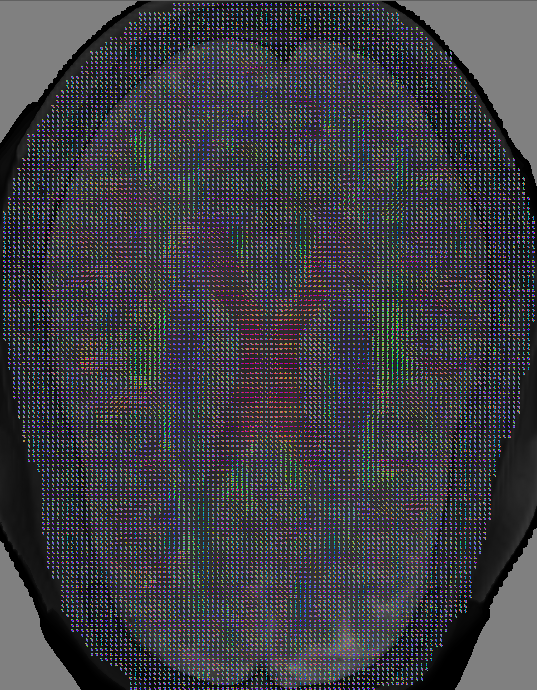
\includegraphics[width=1.0\linewidth, angle=0]{figs/Renderizacao_glifos_evolucao/Adaptividade-multimodal/Fatia_642.png}
      \caption{13205 glifos renderizados sobre um volume \textit{ray-casted}. O glifo é sintetizado a partir da malha esférica obtida pela tesselação de $8^a$ ordem do icosaedro.}
       \label{fig::qualidade_visual_longe_highres}
  %   \hspace{1pt}
 \end{figure}
 
 \textcolor{red}{Ao aplicarmos a estratégia de multi-resolução com base em $max\_p$, obtivemos resultados visualmente similares, porém a um custo computacional menor.}
 
 Fig. \ref{fig::multimodal_162_hollow} e \ref{fig::multimodal_642_hollow} correspondem aos mesmos glifos em Fig. \ref{fig::multimodal_162_filled} e \ref{fig::multimodal_642_filled}, respectivamente e estão apresentados para evidenciar a mudança na quantidade de triângulos em cada um deles. As imagens foram gerada a partir de uma janela $500 \times 500$ com uma diferença sutil no fator de escala entre ambas. 
 
 A resolução dos glifos varia com a utilização da $2^a$ ordem de tesselação do icosaedro (menor nível de detalhe, Fig. \ref{fig::multimodal_lowres}) até a $8^a$ (maior nível de detalhe, Fig. \ref{fig::multimodal_highres}). O FPS do esquema de renderização em função da quantidade de glifos renderizados e parâmetros relacionados de fator de escala e ordem de tesselação utilizados estão listados na Tabela \ref{tab::glyph_info_experiment}, onde atestamos que o algoritmo de renderização proposto integrado ao ambiente de visualização multimodal gera imagens em taxas interativas \cite{nielsen1994}.
 
 \textcolor{red}{Os gráficos na Fig. revelam o comportamento do algoritmo de renderização de glifos proposto quando se varia o fator de escala de visualização, mantendo o nível de resolução das direções e adaptando a resolução conforme o fator de escala da imagem.}
 
 \todo[inline]{Sugiro que plote em gráficos os dados abaixo, para manter a uniformidade, e deslocar os dados numéricos para apêndice ... Seria interessante ter oss dados numéricos de todos os gráficos no apêndice (por uniformidade). Destacar com linhas trajecadas os fatores de escala em que ocorrem transições de ordens de tesselação. }
 
 \todo[inline]{Legenda da Tabela \ref{tab::glyph_info_experiment_fixed} está estranho ... Você quis dizer que a última linha são parâmetros de renderização da Fig. \ref{fig::qualidade_visual_longe_highres}?}

No experimento, integramos o algoritmo à estrutura apresentada no Capítulo \ref{chap::renderizacao_interativa_de_perfis_de_difusao}, no qual algoritmo é integrado ao ambiente multimodal e recebe apenas o conjunto de \textit{voxels} detectados como entrada. O cômputo do parâmetro de ocupância do glifo ($max_p$) efetuado na GPU e o algoritmo de escolha da malha esférica base foram desativados para fins de teste. Adicionalmente, usamos o mesmo volume e métodos descrito na seção \ref{sec::experimentos} do Capítulo \ref{chap::renderizacao_interativa_de_perfis_de_difusao} para gerar os resultados. Os resultados estão apresentados na Tabela \ref{tab::glyph_info_experiment_fixed}.

\begin{table}
\centering
\begin{tabular}{|cccc|}
\hline
\textbf{FPS} & \textbf{Fator de escala} & \textbf{\# glifos} & \textbf{\begin{tabular}[c]{@{}c@{}}Ordem de \\ tesselação\end{tabular}} \\ \hline
34.29 & 86.50 & 12     & 8 \\
35.23 & 58.15 & 20     & 8 \\
35.43 & 38.76 & 42     & 8 \\
35.83 & 25.84 & 90     & 8 \\
32.78 & 17.23 & 182    & 8 \\
35.70 & 11.49 & 380    & 8 \\
32.96 & 7.66  & 870    & 8 \\
28.53 & 5.10  & 1892   & 8 \\
23.17 & 3.40  & 4160   & 8 \\
14.58 & 2.27  & 9166   & 8 \\
 7.96 & 1.51  & 13205  & 8 \\
\hline
\end{tabular}
\caption{Esquema de renderização multimodal com glifos ODF renderizados em uma imagem $850\times 850$ com a malha esférica base fixa. A última linha da tabela descreve a geração da imagem na Fig. \ref{fig::qualidade_visual_longe_highres}.}
\label{tab::glyph_info_experiment_fixed}
\end{table}

\begin{table}[H]
\centering
\begin{tabular}{|cccc|}
\hline
\textbf{FPS} & \textbf{Fator de escala} & \textbf{\# glifos} & \textbf{\begin{tabular}[c]{@{}c@{}}Ordem de \\ tesselação\end{tabular}} \\ \hline
33.85 & 92.27 & 12     & 8 \\
33.69 & 61.51 & 20     & 8 \\
34.75 & 41.01 & 42     & 8 \\
34.66 & 27.34 & 90     & 8 \\
36.29 & 18.23 & 182    & 8 \\
35.97 & 12.15 & 380    & 8 \\
32.98 & 8.10  & 870    & 4 \\
35.83 & 5.40  & 1892   & 4 \\
31.92 & 3.60  & 4160   & 4 \\
22.94 & 2.40  & 9032   & 4 \\
17.15 & 1.52  & 13205  & 2  \\
\hline
\end{tabular}
\caption{Esquema de renderização multimodal com glifos de ODF renderizados em uma imagem $850\times 850$. O número de vértices e triângulos utilizados são computados de acordo com as Eq. \ref{eq::icosphere_vertices} e \ref{eq::icosphere_triangulos}. A Fig. \ref{fig::qualidade_visual_longe_lowres} do apêndice se refere a imagem gerada pelos parâmetros da última linha da tabela}
\label{tab::glyph_info_experiment}
\end{table}

\todo[inline]{Além de não ter selecionado regiões apropriadas (ventrículo lateral !), não é muito clara a visualização dos seus glifos nem RMI-T1 no fundo para as pessoas poderem se contextualizar. Não são nada informativas as Figs. 4.6 e 4.7. Sugiro que faça escolhas melhores. Veja as regiões discutidas em \cite{descoteaux2015}.}

\todo[inline]{A região que você destacou é ventrículo lateral ... Os glifos deveriam ser isotrópicos pois só há liquido cefalorraquidiano ... Dê uma conferida }
\begin{figure}[H]
    \centering
    %\rule{6cm}{3cm}
    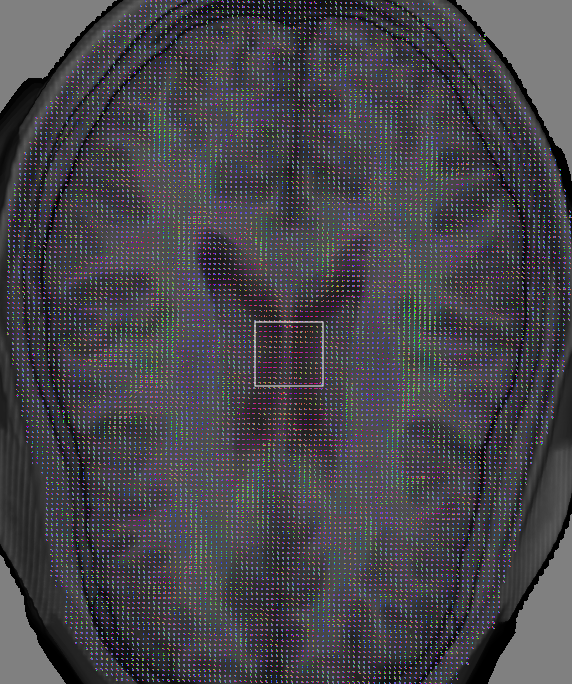
\includegraphics[width=.56\linewidth, angle=0]{figs/Esquema_Glifo/Teste_transicao/base_teste_zoom.png}
    \caption{MRI T1 anatômico co-registrado com DWI. A região dentro do contorno quadrado branco corresponde a região analisada na Fig. \ref{fig::multimodal_teste_zoom}.}
    \label{fig::multimodal_teste_loc}
\end{figure}


\begin{figure}[H]
\centering
\captionsetup[subfloat]{farskip=0pt,nearskip=0pt}
    \subfloat[$4^a$ ordem de tesselação - apenas contornos dos triângulos]{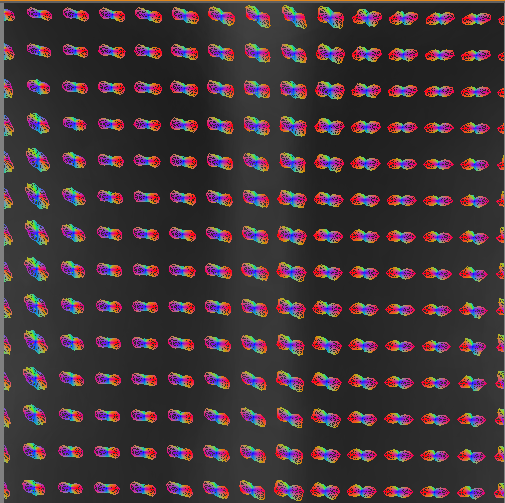
\includegraphics[width=.49\linewidth, angle=0]{figs/Esquema_Glifo/Teste_transicao/162_Hollow.png}
    \label{fig::multimodal_162_hollow}
    }
    \subfloat[$4^a$ ordem de tesselação - triângulos preenchidos] {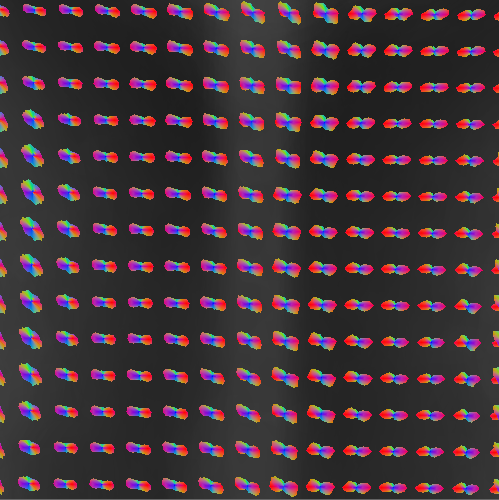
\includegraphics[width=.485\linewidth, angle=0]{figs/Esquema_Glifo/Teste_transicao/162_filled.png}
    \label{fig::multimodal_162_filled}
    }
    \hspace{1pt}
    \subfloat[$8^a$ ordem de tesselação - apenas contornos dos triângulos]{\includegraphics[width=.495\linewidth, angle=0]{figs/Esquema_Glifo/Teste_transicao/642_Hollow.png}
    \label{fig::multimodal_642_hollow}
    }
    \subfloat[$8^a$ ordem de tesselação - triângulos preenchidos] {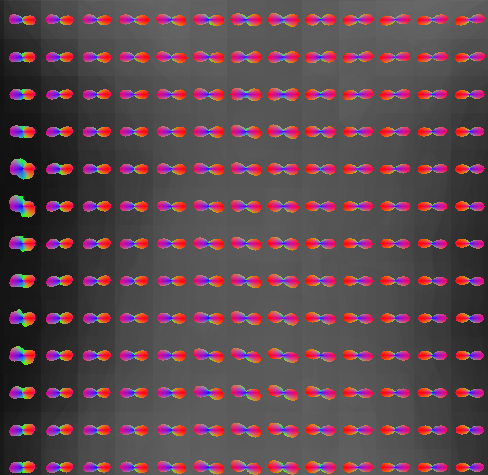
\includegraphics[width=.487\linewidth, angle=0]{figs/Esquema_Glifo/Teste_transicao/642_filled.png}
    \label{fig::multimodal_642_filled}
    }
    \caption{Ilustração da troca de resolução efetuada automaticamente a partir de $max_p$. A troca de resolução ocorre entre as geometrias base derivadas da $4^a$ (\ref{fig::multimodal_162_hollow} e \ref{fig::multimodal_162_filled}) e $8^a$ (\ref{fig::multimodal_642_hollow} e \ref{fig::multimodal_642_filled}) ordem de tesselação. A região ilustrada é do corpo caloso, que está em destaque na Fig. \ref{fig::multimodal_teste_loc}.
    }
    \label{fig::multimodal_teste_zoom}
\end{figure}

\subsection{Discussões}

\todo[inline]{Revisar bem o texto. Está totalmente desconexo.}

Podemos observar a suavidade em que a mudança de resolução ocorre. Observamos que os glifos com os triângulos preenchidos neste nível de resolução não apresentam efeitos característicos de malhas de baixa resolução e que a transição na resolução ocorre de forma sutil. 

 
Adicionalmente, caso o usuário queira analisar os glifos mais de perto ou aumente o tamanho da janela, fazendo-a cobrir mais \textit{pixels}, o glifo é gerado a partir de uma malha suave o suficiente no qual ele tenha total liberdade para visualizar o comportamento das ODFs. Caso o usuário queira ter uma visão mais geral do volume com os glifos e diminua o fator de escala, diminuímos a resolução de cada glifo renderizado para aliviar o processamento computacional associado a cada um deles.

Na Seção \ref{sec::qualidade_visual_longe} do apêndice, apresentamos duas imagens com 13205 glifos onde utilizamos a malha esférica base derivadas da $2^a$ e $8^a$ ordem de tesselação integradas ao ambiente de visualização multimodal, em que estão mapeadas nas Fig. \ref{fig::qualidade_visual_longe_lowres} e \ref{fig::qualidade_visual_longe_highres}, respectivamente. As imagens foram geradas com os parâmetros das últimas linhas das Tabelas \ref{tab::glyph_info_experiment} e \ref{tab::glyph_info_experiment_fixed}, respectivamente. A partir delas, podemos observar que não há diferença visual perceptível, o que nos leva a crer que não há contrapartida em qualidade visual dos glifos para adaptabilidade da malha esférica base.

Na Tabela \ref{tab::glyph_info_experiment} do Capítulo \ref{chap::renderizacao_interativa_de_perfis_de_difusao} consta o experimento feito com a malha esférica adaptativa, e ao comparamos os resultados entre ambas, podemos concluir que conseguimos obter aproximadamente 10 FPS a mais quando 13205 glifos são renderizados e 8,5 FPS quando pouco mais de 9000 glifos são renderizados, e que conseguimos uma solução satisfatória para o problema da interatividade da visualização quando uma grande quantidade de glifos é renderizada.

Há uma diminuição do FPS mostrado nas ultimas duas linhas da tabela \ref{tab::glyph_info_experiment}, onde 9032 e 13205 glifos são renderizados. O gargalo que diminui a performance do algoritmo está relacionada ao alto tráfego de dados GPU-CPU com as coordenadas dos \textit{voxels} detectados. Nesta abordagem de renderização, não podemos compensar este gargalo pois a alta dimensionalidade das ODFs torna inviável o seu armazenamento completo na GPU.

Nas Fig. \ref{fig::multimodal_162_hollow} e \ref{fig::multimodal_162_filled}, o valor de $max_p$ é de 1394 \textit{pixels}, e em \ref{fig::multimodal_642_hollow} e \ref{fig::multimodal_642_filled}, é de 1409. De acordo com Eq. \ref{eq::icosa_order}, o limiar de mudança entre as geometrias é $max_p = 1406.25$.  O glifo mostra uma visão axial do corpo caloso, cujo comportamento de difusão ocorre predominantemente na direção esquerda-direita. Fig. \ref{fig::multimodal_teste_loc} mostra a localização da região mostrada em Fig. \ref{fig::multimodal_teste_zoom}.

%%%%%%%%%%%%%%%%%%%%%%%%%%%%%%%%%%%%%%%%%%%%%%%%%%%%%%%%%%%%%%
\section{Comparações entre Glifos superquádricos e ODFs}
%\section{Glifos ODF integrados ao ambiente de visualização multimodal}
\label{sec::glifos_odf_visualizacao_multimodal}

Propomos um experimento para avaliar aspectos visuais do nosso algoritmo de esquema de renderização em comparação à superquádricas\sout{ e medições de performance para atestarmos a interatividade do algoritmo de renderização} textcolor{red}{quanto à eficácia na revelação das orientações múltiplas das fibras dentro de um voxel}.

\subsection{Descrição}

\textcolor{red}{Sendo o objetivo uma análise visual comparativa entre os glifos superquádricos e os ODFs, geramos com os mesmos volumes usados no segundo experimento (Seção \ref{sec::testes_dados_reais}) os glifos superquádricos propostos por \citeonline{voltoline2021} para uma análise visual comparativa nas formas dos glifos em regiões destacadas por \citeonline{descoteaux2015}.}

\subsection{Resultados}

\todo[inline]{Talvez seja interessante em destacar os glifos ODFs com mais pontas ... Não dá para perceber nas figuras. Use por exemplo o package tikz. Acho que o Wallace usou muito na tese dele ...}

\textcolor{red}{Mostraremos comparativamente as imagens com os glifos superquádricos geradas com as imagens selecionadas na seção \ref{ssec::reais_resultados}.}

Fig. \ref{fig::multimodal} ilustra uma fatia coronal na região do \textit{centrum semiovale} com um triplo cruzamento de fibras correspondentes do corpo caloso, \textit{corona radiata} e o fascículo longitudinal superior. A região apresenta cruzamentos de fibra conhecidos e é utilizada para análises qualitativas. Fig. \ref{fig::multimodal_highres} mostra que pode-se inferir sobre cada cruzamento de fibra nas regiões mais alongadas da superfície do glifo. Observe também que a resolução do glifo é diferente na Fig. \ref{fig::multimodal_lowres} em comparação a \ref{fig::multimodal_highres} e sua seleção é feita de forma automática. No fundo, há a renderização da ressonância anatômica ponderada em T1 co-registrada.

\begin{figure}[H]
\centering
%\captionsetup[subfloat]{farskip=0pt,nearskip=0pt}
    %\rule{6cm}{3cm}
    \subfloat[]{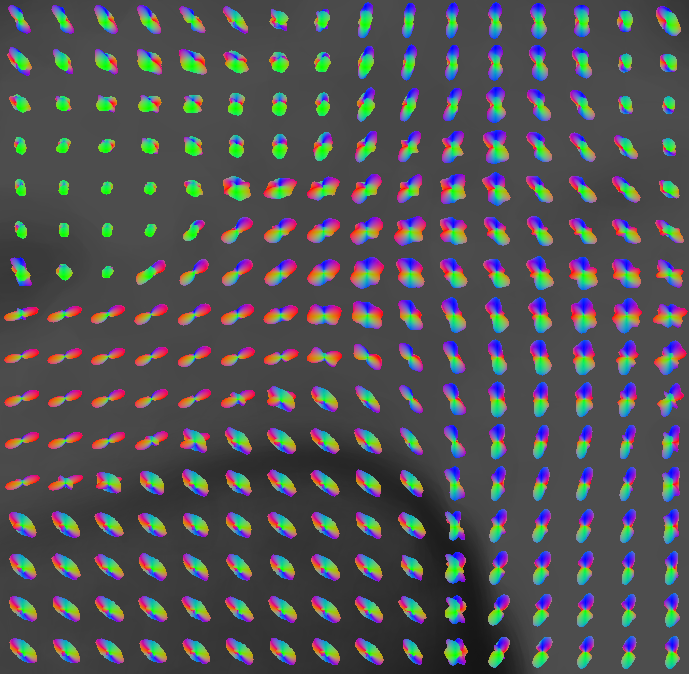
\includegraphics[width=.45\linewidth, angle=0]{figs/Esquema_Glifo/HighResImg.png}
    \label{fig::multimodal_highres}}
    \subfloat[] {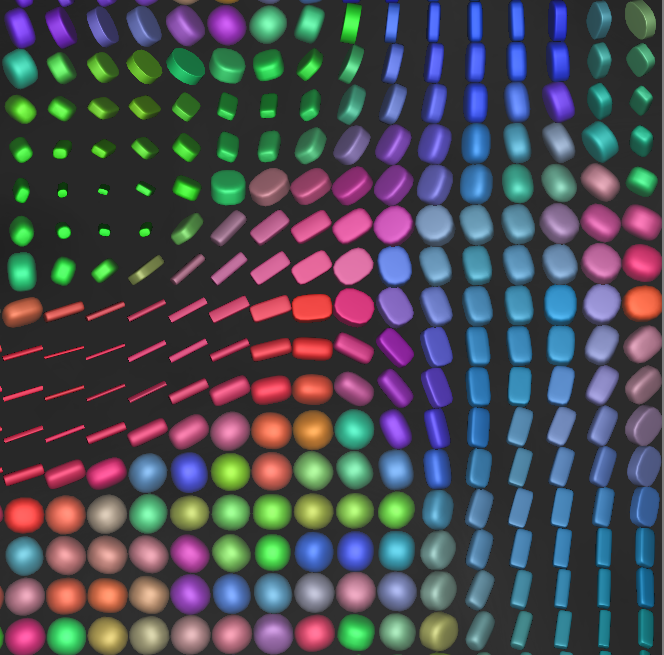
\includegraphics[width=.45\linewidth, angle=0]{figs/Esquema_Glifo/HighResImgSuperquadric.png}
    \label{fig::multimodal_superq}}
    \caption{Configurações das fibra na região de cruzamento dos tratos CS, SLF e CC.}
    \label{fig::multimodal_superquadric}
\end{figure}


\subsection{Discussões}

\todo[inline]{Revise integralmente o texto. Os glifos mostrados no link realçam melhor as direções (fODFs)! \url{http://cmic.cs.ucl.ac.uk/cdmri10/invited_tournier.pdf}. É preciso levar em conta nas discussões}

\citeonline{voltoline2021} evidenciaram que a sua respectiva renderização multimodal para superquádricas do DTI pode ajudar no processo de escolhas referentes a sementes em tractografia, em comparação à mapas de anisotropia codificados por cor. Fig. \ref{fig::multimodal_superquadric} ilustra a mesma região de Fig. \ref{fig::multimodal_highres} com superquádricas. Note que os glifos apresentam o mesmo problema presente no próprio DTI: em cruzamentos de fibra, a distribuição de fibras subjacente não é inferível. Pode-se perceber isto na região de cruzamento de fibras enquanto nos glifos ODF, é possível inferir sobre a natureza do cruzamento de fibras, nas superquádricas, o glifo apresenta uma forma retangular suave e não gera a possibilidade de inferir sobre as fibras que compõem o cruzamento.




%%%%%%%%%%%%%%%%%%%%%%%%%%%%%%%%%%%%%%%%%%%%%%55555


%\subsection{Renderização por Fatias}
%\label{ssec::renderizacao_por_fatias}

%Podemos comparar nossa abordagem com a de \citeonline{shattuck2008}, uma vez que ambas são baseadas em polígonos, onde amostras de ODF deformam uma malha esférica. Em sua abordagem, \citeonline{shattuck2008} armazena ODFs como coeficientes de funções base na CPU e os glifos são computados e visualizados em fatias, que são visualizadas de forma ortogonal. O cômputo da forma dos glifos é feito na CPU, onde o valor de ODF é computada para as normais dos vértices da malha esférica utilizada, deslocando cada um dos vértices, e o tráfego CPU-GPU consiste no envio de dados de vértices de forma que sua estrutura de dados define a superfície do glifo.

%Em nossa abordagem, setamos a malha esférica de amostragem a priori e armazenamos amostras de dados de ODF e mostramos estratégias para escolher a malha esférica adequada e estratégias para lidar com o gargalo de tráfego de dados CPU-GPU. Para atingir este objetivo, mostramos formas de organizar os dados de ODF e da malha esférica de amostragem para utilizar renderização por instâncias, técnica que não estava disponível quando \citeonline{shattuck2008} publicaram seu trabalho\footnote{Em OpenGL, renderização por instâncias foi disponibilizada a partir da versão 3.2, lançada em 2009}. Adicionalmente, no processo de renderização, apenas enviamos um conjunto de escalares de ODF para deslocar a malha esférica escolhida e deslocamos os pontos da malha nas \textit{threads} da GPU. Assim, o tráfego de dados por glifo é de $N/2 + (4-N/2 \mod{4})$ \textit{floats} para uma geometria base com $N$ vértices. A possibilidade de diminuir o tráfego de dados por glifo para esta quantidade tem sido crucial para renderizar este glifos com malhas suaves em taxas interativas. Adicionalmente, os glifos são renderizados com apenas um comando de desenho e sua quantidade máxima é limitada pelo máximo número de elementos permitidos em uma das dimensões da textura 2D.

%Uma vez que nossa abordagem é vinculada à renderização de um volume via \textit{ray-casting}, apenas os \textit{voxels} visíveis são requisitados a serem desenhados, e não há a restrição a uma fatia inteira. Além disso, no ambiente interativo de visualização, onde o usuário tem a possibilidade de mudar a escala e mover o volume, a detecção de \textit{voxels} visíveis certifica que os \textit{voxels} que estão fora da cena não são demandados na renderização, consequentemente, seus dados não são enviados à GPU e nem são processados no \textit{vertex shader} para serem descartados na rasterização.

%Nosso esquema é também aplicável em renderização de glifos baseada em fatia. Observe que, o conjunto $D$ pode se referir a um conjunto de índices referentes a \textit{voxels} que definem uma fatia. Adicionalmente, os atributos de translação podem posicionar os glifos em um \textit{grid} $W \times H$, onde este atributo posiciona cada objeto ao centro de cada célula, que é escalonado pelo fator que o faz estar contido.

%Objetivando gerar resultados de performance do algoritmo e renderização em uma fatia 2-D, fizemos o seguinte experimento: os eixos x e y são divididos em $H$ intervalos ($W = H$), gerando o total de $H^2$ células quadriculadas, no qual glifos são renderizados em cada uma delas. Cada glifo é escalonado para estar contido em sua respectiva célula e posicionado em seu centro. Fixamos a geometria base, assim como os atributos de translação e, para evidenciar a interatividade do algoritmo sob a circunstância de uma frequente troca de fatias, a cada requisição de desenho, os atributos de translação e a matriz de amostras de ODF são preparados e enviados à GPU, conforme mostrado na Subseção \ref{ssec::atributos}.

%Mensuramos o FPS como uma função da quantidade de glifos renderizados com $H$ variando de 5 até 100. O gráfico de $FPS \times \text{glifos renderizados}$ é ilustrado na Fig. \ref{fig::slice_benchmark} para diferentes geometria base utilizadas em uma janela $1200\times 1200$.

% \begin{figure}[htb]
%     \centering
%     %\rule{6cm}{3cm}
%     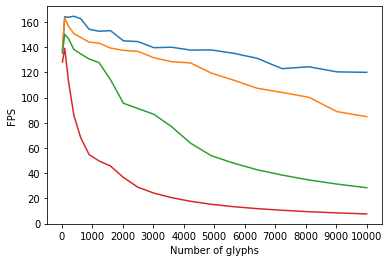
\includegraphics[width=.65\linewidth, angle=0]{figs/Esquema_Glifo/benchmark_half_texopt.png}
%     \caption{FPS $\times$ quantidade de glifos renderizada. As cores azul, laranja, verde e vermelha correspondem a geometria base gerada pela $2^{a}$ $4^{a}$, $8^{a}$ e $16^{a}$ ordem de tesselação do icosaedro. Suas respectivas quantidades de vértices e triângulo são computadas nas Eq. \ref{eq::2ordem_icosphere_vertices} e \ref{eq::2ordem_icosphere_triangulos}, respectivamente.}
%     \label{fig::slice_benchmark}
% \end{figure}

%Os resultados indicam que nosso esquema dá resultados satisfatórios para uso interativo, e mostramos que é possível renderizar milhares de glifos em taxas interativas utilizando a $4^{a}$ ordem de tesselação do icosaedro e centenas com a malha suave gerada pela $16^{a}$ ordem de tesselação.

%Na próxima seção, descrevemos uma infra-estrutura fora do ambiente de renderização multimodal para renderização de glifos ODF no qual a utilizamos para fazer testes e validações da melhora do algoritmo. Nela, apresentamos o primeiro protótipo do algoritmo, no qual tem semelhanças com o trabalho de \citeonline{shattuck2008} e as funcionalidades adicionadas ao longo do tempo. Para mensurar ganhos obtidos para cada funcionalidade adicionada, mensuramos o FPS do algoritmo para diferentes quantidade de glifos renderizadas para diferentes resoluções e comparamos com à abordagem anterior.

%Objetivando gerar resultados de performance do algoritmo e renderização em uma fatia 2-D, fizemos o seguinte experimento: os eixos x e y são divididos em $H$ intervalos ($W = H$), gerando o total de $H^2$ células quadriculadas, no qual glifos são renderizados em cada uma delas. Cada glifo é escalonado para estar contido em sua respectiva célula e posicionado em seu centro. Fixamos a geometria base, assim como os atributos de translação e, para evidenciar a interatividade do algoritmo sob a circunstância de uma frequente troca de fatias, a cada requisição de desenho, os atributos de translação e a matriz de amostras de ODF são preparados e enviados à GPU, conforme mostrado na Subseção \ref{ssec::atributos}.


%, no qual foi aperfeiçoado por \cite{almsick2011}. Esta abordagem possibilitou incrementos em performance em relação a \citeonline{shattuck2008}.

%\citeonline{raphael_dissertacao} propôs um esquema de renderização interativa do tensor de difusão em glifos superquádricos \cite{Kindlmann2004} utilizando polígonos. Em seu trabalho, os glifos são renderizados a taxas interativas e a sua abordagem consiste na minimização de tráfego de dados entre CPU-GPU, que consiste apenas em parâmetros que customizam e deslocam os glifos, e o uso de renderização por instâncias. Adicionalmente, este esquema está integrado ao VMTK-Neuro. Os resultados obtidos neste trabalho nos influenciou a adaptar o seu esquema para glifos HARDI.



%\subsection{\sout{Abordagem de renderização}}

%\sout{\citeonline{peeters2009} apresentou pela primeira vez um esquema de renderização para esta categoria de glifos, nos quais são aperfeiçoados por \citeonline{almsick2011} e \citeonline{hlawitschka2012}. Estes esquemas utilizam a abordagem \textit{raycasting}.}

%\sout{No VMTK-Neuro, um dos algoritmos de renderização do tensor difusão por glifos superquádricos é feita por instanciações de uma malha esférica, no qual é customizada por parâmetros particulares a cada tensor de difusão referentes a cada \textit{voxel} detectado e posicionado na cena de acordo. Este esquema de renderização desenha os glifos em tempo interativo.}

%\sout{Pela maior simplicidade e boa efetividade da renderização por instanciações de uma malha esférica, o esquema desenvolvido neste trabalho utiliza esta abordagem.}



%Dados relativos ao desempenho \sout{serão mais detalhados na dissertação de mestrado}\textcolor{blue}{estão disponíveis no link ...}.



%\sout{Medições do tempo relativo ao desempenho foram feitas para a quantidade de 197 vértices da malha esférica \sout{em um}\textcolor{blue}{num} volume de resolução 128x128x90. Para uma quantidade na faixa de 5000 glifos renderizados simultaneamente sobre uma fatia completa, obtemos tem um tempo de resposta entre 80 e 110ms. Para uma quantidade pequena de glifos na faixa das dezenas, o tempo de resposta cai para o intervalo entre 60 e 70ms. Esse tempo de resposta está nas proximidades ou é menor do que o tempo de 0,1s, que é o limite máximo para que o usuário tenha a percepção de resposta instantânea da máquina e que suas ações são a causa de que algo aconteça na tela \cite{nielsen1994}.}

%\sout{No cômputo das ODFs do \textit{QBall}, é feito o mapeamento do sinal de DWI para a ODF a partir das direções derivadas da malha esférica. O glifo para visualização é gerado diretamente de acordo a representação gráfica polar esférica em que $R(\textbf{u}) = R(\mathbf{u})$, onde \textbf{u} é a direção de difusão. A malha esférica utilizada para geração dos glifos em \ref{section::QBall_Glifos} está representada na figura \ref{fig::MalhaEsferico}.}

%A priori, todas as ODFs são calculadas e normalizadas para o intervalo $[0,1]$ para cada um dos \textit{voxels} do volume e referenciadas no processo de renderização.

%O formato de armazenamento dos valores ODF associados à malha consiste numa lista de valores escalares associados a cada um dos \textit{voxels}.



%\todo[inline]{Falta uma descrição melhor de como são construídos os glifos a partir de ODFs e o seu mapeamento às entidades gráficas. Isso torna difícil o entendimento da sua implementação. !!Descrito em trabalhos relacionados!}
